%==============================================================
%  Laporan Tugas Besar  EL4045 Komputasi Performa Tinggi
%  Solver Rangkaian MNA Paralel (Sekuensial / OpenMP / OpenCL)
%  Format: IEEE (IEEEtran, conference)
%==============================================================
\documentclass[conference]{IEEEtran}
\IEEEoverridecommandlockouts

\usepackage[T1]{fontenc}
\usepackage[utf8]{inputenc}
\usepackage{amsmath,amssymb,amsfonts}
\usepackage{graphicx}
\usepackage{booktabs}
\usepackage{array}
\usepackage{xcolor}
\usepackage{listings}
\usepackage[ruled,vlined,linesnumbered]{algorithm2e}
\usepackage{siunitx}
\usepackage{textcomp}
\usepackage[hidelinks]{hyperref}

\sisetup{group-separator={.},output-decimal-marker={,}}

% --- gaya listing kode ---
\definecolor{codegray}{gray}{0.95}
\definecolor{codekw}{rgb}{0.10,0.30,0.65}
\definecolor{codecm}{rgb}{0.35,0.55,0.35}
\lstset{
  basicstyle=\ttfamily\footnotesize,
  keywordstyle=\color{codekw}\bfseries,
  commentstyle=\color{codecm}\itshape,
  backgroundcolor=\color{codegray},
  breaklines=true, frame=single, framesep=3pt,
  columns=fullflexible, showstringspaces=false,
  numbers=none, aboveskip=4pt, belowskip=2pt, xleftmargin=2pt
}

\begin{document}

\title{Akselerasi Paralel Penyelesaian Sistem Linear Analisis Nodal Termodifikasi (MNA) Menggunakan OpenMP dan OpenCL}

\author{
\IEEEauthorblockN{Fairuz Apuilla Rahagi\IEEEauthorrefmark{1},
Adam Mohammad Febrian\IEEEauthorrefmark{2},
Ahmad Ramadhan\IEEEauthorrefmark{3}}
\IEEEauthorblockA{Sekolah Teknik Elektro dan Informatika\\
Institut Teknologi Bandung, Bandung, Indonesia\\
Email: \IEEEauthorrefmark{1}13222107@mahasiswa.itb.ac.id,
\IEEEauthorrefmark{2}13222015@mahasiswa.itb.ac.id,
\IEEEauthorrefmark{3}13222110@mahasiswa.itb.ac.id}
}

\maketitle

\begin{abstract}
Pada dasarnya, simulasi rangkaian elektrik dapat direduksi menjadi penyelesaian sistem persamaan linear $A\mathbf{x}=\mathbf{b}$ yang dibangun melalui metode \emph{Modified Nodal Analysis} (MNA). Inti komputasinya, yakni dekomposisi LU pada matriks padat, memiliki kompleksitas $O(n^3)$ dan menjadi penghambat utama (\emph{bottleneck}) ketika ukuran rangkaian membesar. Makalah ini memaparkan rancangan dan implementasi sebuah solver MNA yang menyelesaikan sistem linear tersebut dengan tiga \emph{backend} berbeda: sekuensial satu inti, paralel multi-inti berbasis OpenMP, dan paralel GPU berbasis OpenCL. Ketiganya menggunakan algoritma dekomposisi LU yang identik secara matematis sehingga perbandingan kinerjanya benar-benar setara. Kebenaran solver divalidasi terhadap nilai analitik dan terhadap simulator komersial LTspice. Hasil pengujian (\emph{benchmark}) pada matriks berukuran $n=51$ hingga $n=1001$ memperlihatkan adanya fenomena \emph{crossover} yang khas: untuk matriks kecil seluruh backend paralel justru lebih lambat akibat ongkos paralelisasi, dan paralelisasi baru memberikan keuntungan ketika $n \gtrsim 500$. Pada $n=1001$ diperoleh percepatan tertinggi $2{,}64\times$ (OpenMP 4 utas) dan $2{,}35\times$ (OpenCL, waktu komputasi). Temuan ini menegaskan prinsip dasar komputasi performa tinggi: paralelisasi selalu menuntut ongkos, dan baru menguntungkan apabila volume kerja cukup besar untuk menutupi \emph{overhead} tersebut.
\end{abstract}

\begin{IEEEkeywords}
komputasi performa tinggi, analisis nodal termodifikasi, dekomposisi LU, OpenMP, OpenCL, GPU, paralelisasi
\end{IEEEkeywords}

%==============================================================
\section{Pendahuluan}
%==============================================================
Penyelesaian sistem persamaan linear merupakan kernel komputasi yang muncul di hampir seluruh cabang sains dan rekayasa: analisis elemen hingga, pemrosesan sinyal, pembelajaran mesin, hingga simulasi rangkaian elektrik. Pada simulasi rangkaian, perangkat lunak kelas SPICE membangun model matematis rangkaian, lalu menyelesaikan sistem $A\mathbf{x}=\mathbf{b}$ untuk memperoleh tegangan tiap simpul dan arus tiap sumber~\cite{nagel1975spice}. Ketika jumlah simpul bertambah, biaya penyelesaian sistem inilah yang mendominasi keseluruhan waktu simulasi.

Mata kuliah Komputasi Performa Tinggi menekankan bagaimana sebuah persoalan komputasi yang \emph{compute-bound} dapat dipercepat dengan memanfaatkan paralelisme perangkat keras modern, baik berupa banyak inti CPU maupun ribuan inti GPU. Atas dasar itu, tim memilih persoalan penyelesaian sistem linear MNA sebagai studi kasus, karena: (i) persoalan ini nyata dan dapat diverifikasi terhadap perangkat lunak komersial; (ii) kernel komputasinya, dekomposisi LU padat, adalah \emph{benchmark} paralel kanonik yang sama dengan yang dipakai LINPACK untuk memeringkat superkomputer dunia~\cite{dongarra2003linpack}; dan (iii) persoalan ini bukan persoalan pengurutan (\emph{sorting}), sesuai batasan tugas.

Kontribusi makalah ini adalah: (1) perumusan dan implementasi pembangun matriks MNA lengkap dengan mekanisme \emph{stamping}; (2) tiga implementasi solver LU yang identik secara algoritmik namun berbeda strategi paralelisasinya (sekuensial, OpenMP, OpenCL); (3) kerangka pengujian otomatis yang memvalidasi kebenaran dan mengukur kinerja; serta (4) analisis menyeluruh atas perilaku percepatan, termasuk fenomena \emph{crossover} dan keterbatasan skalabilitas.

%==============================================================
\section{Permasalahan Komputasi}
%==============================================================
\subsection{Rumusan Persoalan}
Diberikan sebuah rangkaian linear yang terdiri atas resistor, sumber tegangan, dan sumber arus, persoalannya adalah mencari potensial tiap simpul (relatif terhadap simpul referensi/ground) dan arus cabang tiap sumber tegangan. Dengan metode MNA, persoalan fisis ini diubah menjadi sistem linear
\begin{equation}
A\mathbf{x}=\mathbf{b}, \qquad A\in\mathbb{R}^{n\times n},\; \mathbf{x},\mathbf{b}\in\mathbb{R}^{n},
\label{eq:axb}
\end{equation}
dengan $n=(N-1)+M$, di mana $N$ adalah jumlah simpul (termasuk ground) dan $M$ adalah jumlah sumber tegangan. Vektor solusi $\mathbf{x}$ memuat $N-1$ tegangan simpul disusul $M$ arus cabang.

\subsection{Karakteristik Komputasi}
Penyelesaian \eqref{eq:axb} melalui eliminasi Gauss / dekomposisi LU membutuhkan sekitar $\tfrac{2}{3}n^3$ operasi \emph{floating-point}, sementara substitusi maju-mundur hanya $O(n^2)$. Dengan demikian, untuk $n$ besar, tahap faktorisasi LU mendominasi total komputasi. Sifat $O(n^3)$ inilah yang menjadikan persoalan ini bersifat \emph{compute-bound} sekaligus menjadi target ideal untuk paralelisasi: setiap kali $n$ digandakan, beban kerja meningkat delapan kali lipat. Perlu dicatat bahwa persoalan ini sama sekali tidak melibatkan pengurutan; beban komputasinya murni aljabar linear numerik.

%==============================================================
\section{Solusi yang Telah Ada}
%==============================================================
Penyelesaian sistem linear dari analisis rangkaian merupakan persoalan klasik dengan beragam solusi mapan.

\textbf{Simulator SPICE.} Perangkat lunak seperti SPICE~\cite{nagel1975spice} dan turunannya (LTspice, ngspice) menggunakan MNA yang dipasangkan dengan pemfaktoran LU jarang (\emph{sparse LU}). Pendekatan ini sangat efisien untuk rangkaian nyata yang matriksnya didominasi nol.

\textbf{Pustaka aljabar linear padat.} LAPACK dan BLAS menyediakan rutin faktorisasi LU padat (mis. \texttt{dgetrf}) yang teroptimasi tinggi terhadap hierarki memori melalui algoritma berblok~\cite{golub2013matrix}. \emph{Benchmark} LINPACK yang dibangun di atasnya menjadi tolok ukur resmi peringkat TOP500~\cite{dongarra2003linpack}.

\textbf{Solver jarang.} Untuk matriks jarang, pustaka seperti KLU dan SuiteSparse~\cite{davis2010klu} mengeksploitasi struktur nol sehingga menghindari komputasi yang sia-sia. Khusus matriks tridiagonal, algoritma Thomas menyelesaikan sistem dalam $O(n)$.

\textbf{Akselerasi GPU.} Pustaka seperti cuSOLVER dan MAGMA menyediakan faktorisasi LU pada GPU, memanfaatkan ribuan inti untuk mengakselerasi operasi level matriks~\cite{stone2010opencl}.

Solusi-solusi komersial dan pustaka ini sangat matang, namun bersifat \emph{black box} sehingga kurang sesuai untuk tujuan pembelajaran. Untuk tujuan tugas ini, tim membangun solver dari nol agar dapat mengontrol dan membandingkan strategi paralelisasi secara langsung, dengan LTspice diposisikan sebagai acuan kebenaran (\emph{ground truth}).

%==============================================================
\section{Alternatif Solusi Tim}
%==============================================================
Tim mengusulkan tiga implementasi solver yang menyelesaikan persoalan yang sama, \eqref{eq:axb}, dengan algoritma dekomposisi LU yang identik, tetapi berbeda pada strategi pemetaan komputasi ke perangkat keras. Strategi ini diringkas pada Tabel~\ref{tab:strategi}.

\begin{table}[t]
\caption{Tiga Alternatif Strategi Paralelisasi}
\label{tab:strategi}
\centering
\renewcommand{\arraystretch}{1.25}
\begin{tabular}{@{}p{1.45cm}p{2.0cm}p{3.5cm}@{}}
\toprule
\textbf{Backend} & \textbf{Paralelisme} & \textbf{Catatan} \\
\midrule
Sekuensial & Tidak ada & LU + \emph{partial pivoting} di CPU; menjadi \emph{baseline}. \\
OpenMP & Multi-inti CPU & \texttt{\#pragma omp parallel for} pada perulangan eliminasi baris; \texttt{schedule(dynamic)}; pivoting tetap sekuensial. \\
OpenCL & Banyak inti GPU & Dua kernel 1D/2D per kolom pivot; tanpa pivoting; hasil diverifikasi via residu. \\
\bottomrule
\end{tabular}
\end{table}

\textbf{Sekuensial} berfungsi sebagai garis dasar yang benar dan stabil secara numerik. \textbf{OpenMP} mendistribusikan perulangan eliminasi baris (yang antar-barisnya saling bebas) ke beberapa utas CPU dengan ongkos perubahan kode minimal. \textbf{OpenCL} memetakan tiap sel sub-matriks aktif ke satu \emph{work-item} GPU, mengeksploitasi paralelisme data masif namun dengan ongkos transfer data host$\leftrightarrow$device dan tanpa pivoting (yang sukar diimplementasikan secara efisien di GPU).

%==============================================================
\section{Desain Sistem}
%==============================================================
\subsection{Arsitektur Sistem}
Sistem dirancang sebagai alur pemrosesan berlapis (Gambar~\ref{fig:arch}): \emph{lapisan masukan} membangun objek rangkaian; \emph{lapisan model} mengubah rangkaian menjadi matriks MNA; \emph{lapisan komputasi} menyelesaikan sistem linear dengan salah satu dari tiga backend; dan \emph{lapisan keluaran} memverifikasi serta melaporkan hasil. Pemisahan ini membuat ketiga solver dapat dipertukarkan tanpa mengubah bagian pembangun matriks.

\begin{figure*}[t]
\centering
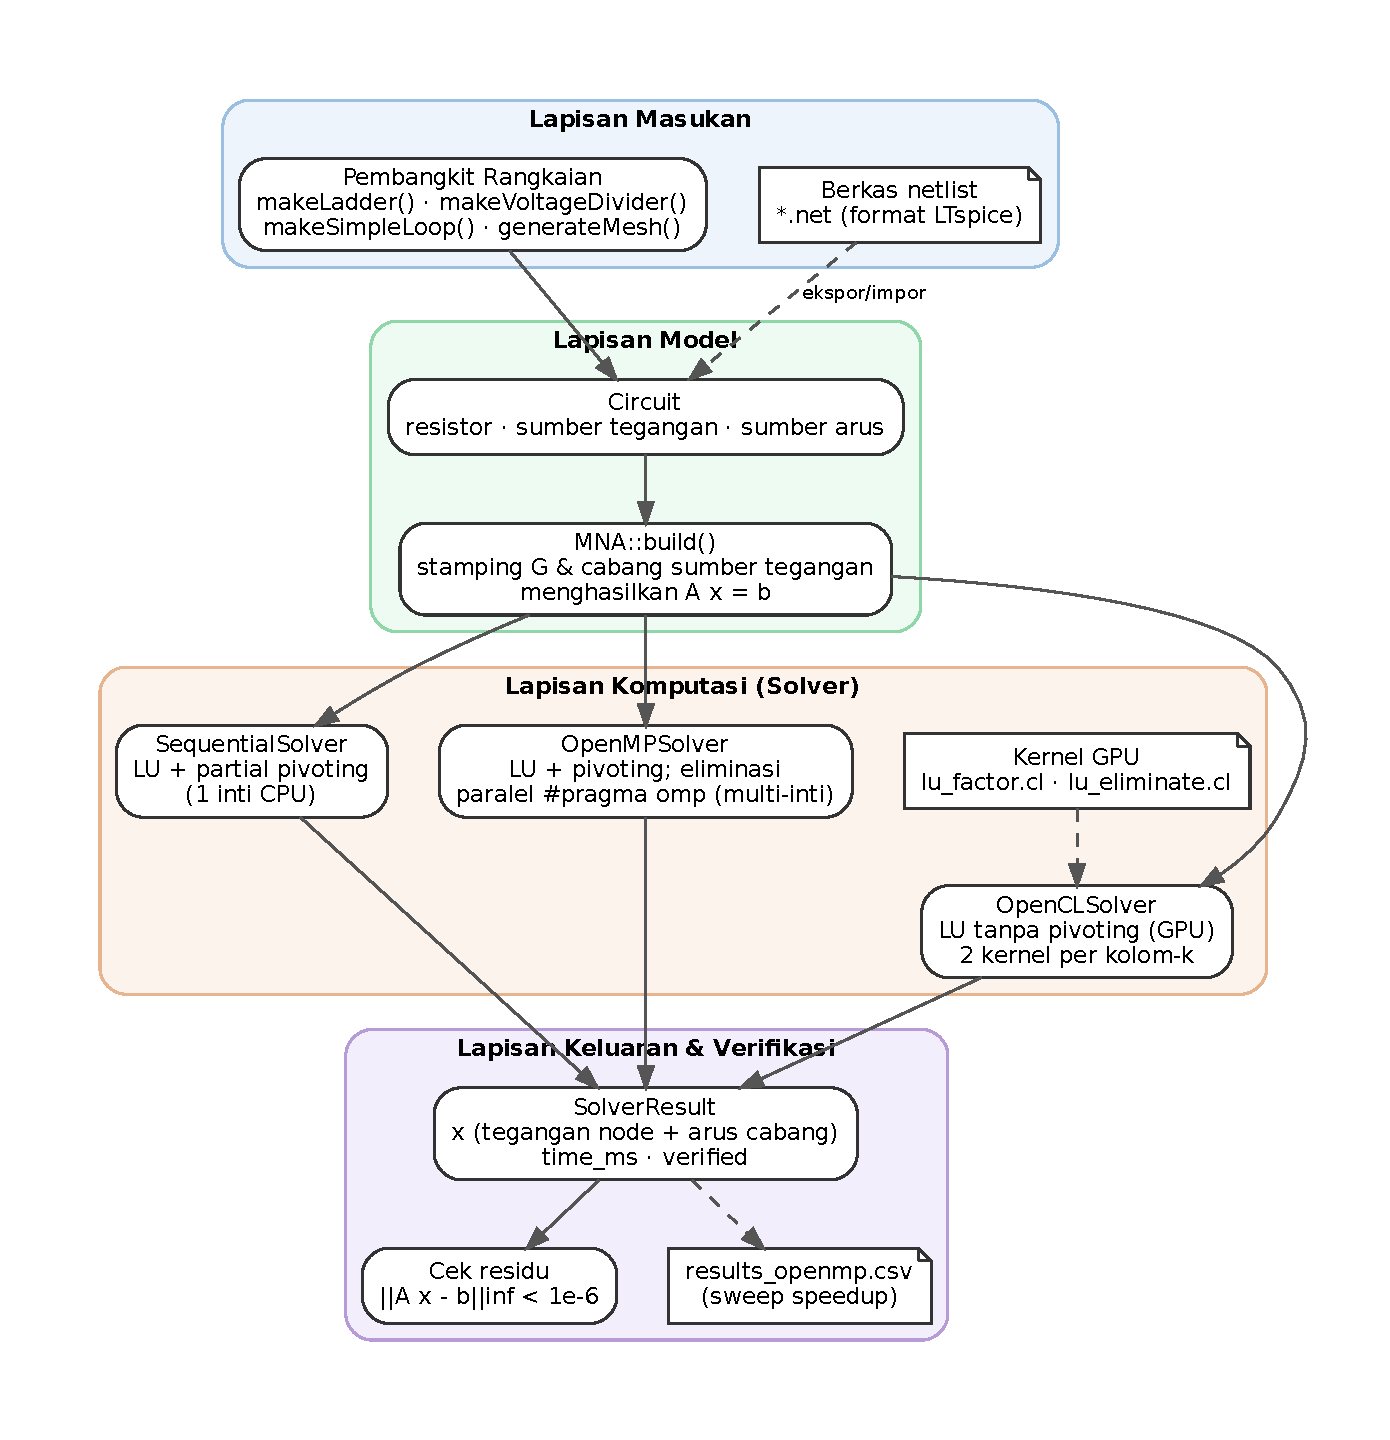
\includegraphics[width=0.92\textwidth]{fig/arch.pdf}
\caption{Arsitektur sistem solver MNA paralel. Pembangun matriks MNA bersifat tunggal, sementara ketiga backend solver dapat dipertukarkan dan menghasilkan struktur \texttt{SolverResult} yang seragam.}
\label{fig:arch}
\end{figure*}

\subsection{Diagram Aliran Data (DFD)}
Diagram konteks (DFD level~0) pada Gambar~\ref{fig:dfd0} menempatkan sistem sebagai satu proses tunggal yang berinteraksi dengan dua entitas eksternal: \emph{Pengguna} (yang memberi parameter rangkaian dan menerima hasil) dan \emph{LTspice} (sebagai sumber tegangan referensi untuk validasi). Diagram level~1 pada Gambar~\ref{fig:dfd1} memecah sistem menjadi empat proses: (1) membangun rangkaian, (2) menyusun matriks MNA, (3) menyelesaikan sistem linear, dan (4) memverifikasi serta melaporkan hasil; ditambah tiga penyimpanan data: berkas kernel GPU, berkas hasil \emph{benchmark}, dan berkas netlist.

\begin{figure}[t]
\centering
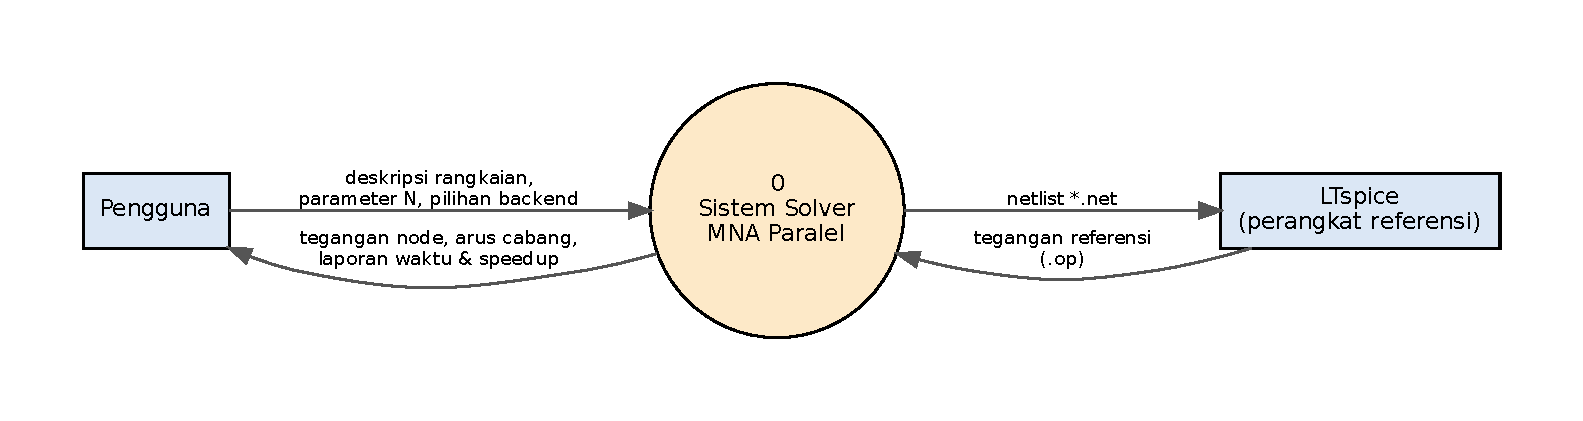
\includegraphics[width=\columnwidth]{fig/dfd0.pdf}
\caption{DFD level~0 (diagram konteks).}
\label{fig:dfd0}
\end{figure}

\begin{figure*}[t]
\centering
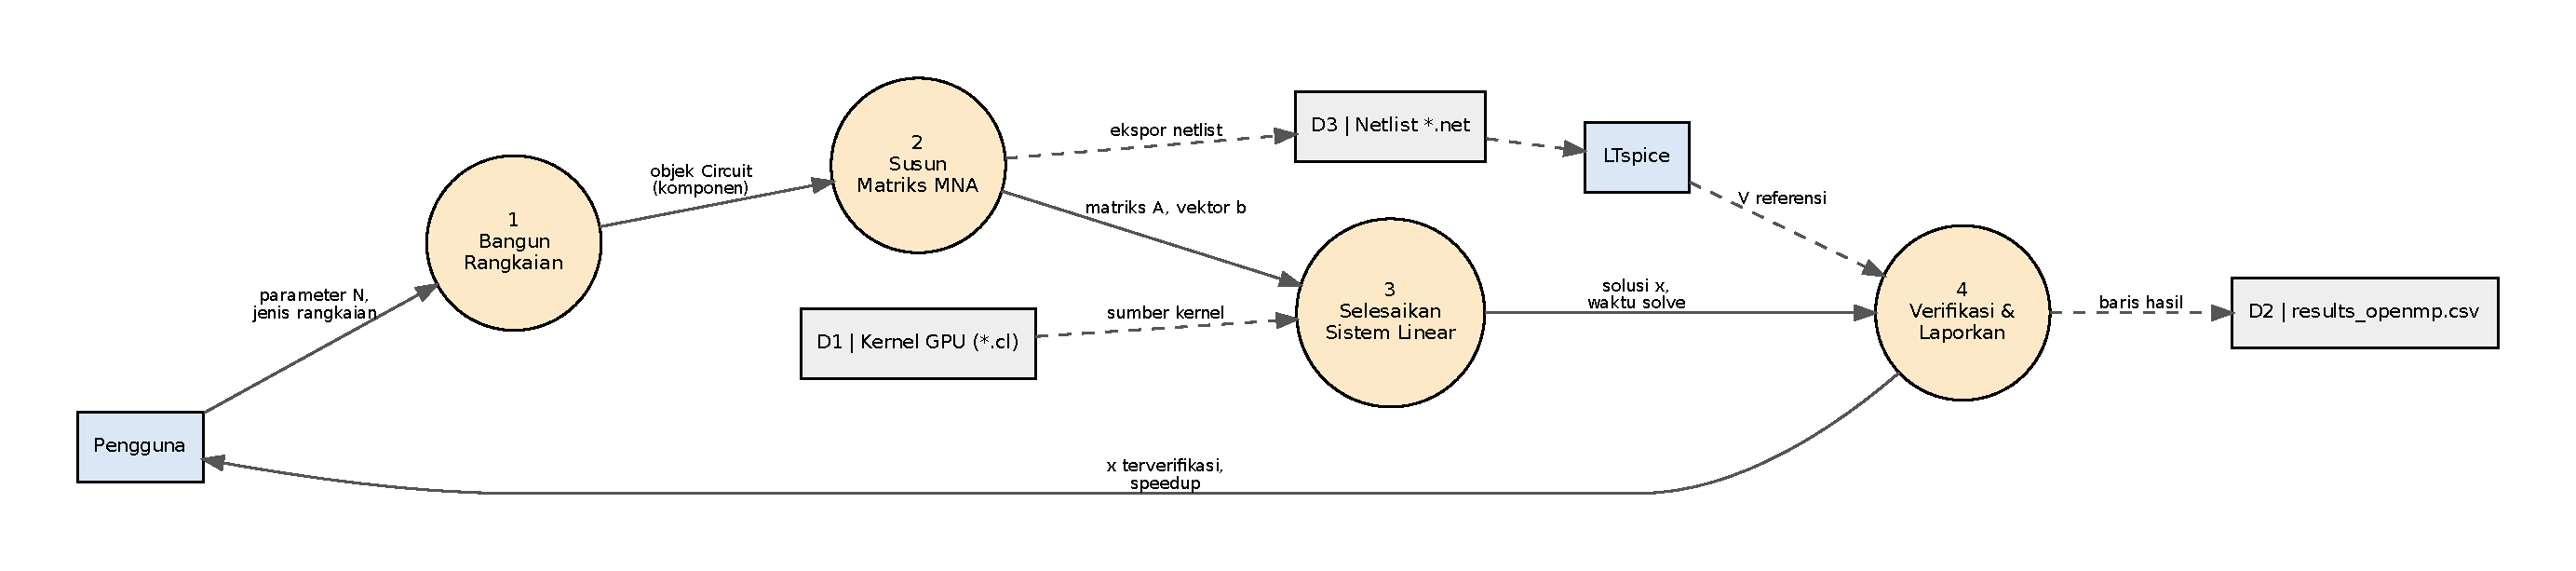
\includegraphics[width=0.95\textwidth]{fig/dfd1.pdf}
\caption{DFD level~1: empat proses utama beserta aliran data dan penyimpanan data.}
\label{fig:dfd1}
\end{figure*}

\subsection{Formulasi MNA dan Aturan \emph{Stamping}}
Matriks MNA dibangun melalui mekanisme \emph{stamping}: tiap komponen menyumbangkan kontribusi ke sel-sel tertentu dari $A$ dan $\mathbf{b}$. Untuk resistor dengan konduktansi $G=1/R$ antara simpul $i$ dan $j$ (indeks digeser karena simpul ground tidak masuk matriks):
\begin{equation}
A_{ii}\!\mathrel{+}=\!G,\;\; A_{jj}\!\mathrel{+}=\!G,\;\; A_{ij}\!\mathrel{-}=\!G,\;\; A_{ji}\!\mathrel{-}=\!G.
\end{equation}
Untuk sumber tegangan ke-$k$ bernilai $V_k$ antara simpul $p$ dan $q$, ditambahkan satu baris/kolom cabang berindeks $r=(N-1)+k$:
\begin{equation}
A_{pr}=A_{rp}=+1,\quad A_{qr}=A_{rq}=-1,\quad b_r=V_k,
\end{equation}
sedangkan sumber arus $I$ menyumbang $b_p\mathrel{+}=I$ dan $b_q\mathrel{-}=I$. Potongan inti rutin \emph{stamping} ditunjukkan pada Listing~\ref{lst:stamp}.

\begin{lstlisting}[language=C++,caption={Inti rutin stamping MNA (\texttt{mna.cpp}).},label={lst:stamp}]
double G = 1.0 / r.resistance;
if (i>0) A[i-1][i-1] += G;
if (j>0) A[j-1][j-1] += G;
if (i>0 && j>0) {
  A[i-1][j-1] -= G;
  A[j-1][i-1] -= G;
}
\end{lstlisting}

\subsection{Algoritma LU dan Diagram Alir}
Ketiga backend menjalankan dekomposisi LU yang sama: untuk tiap kolom pivot $k$, dipilih pivot terbesar (pivoting parsial, hanya pada jalur CPU), baris ditukar, lalu seluruh baris di bawah pivot dieliminasi. Tahap eliminasi inilah yang diparalelkan. Algoritma~\ref{alg:lu} merangkum prosedurnya, dan Gambar~\ref{fig:flow} menyajikan diagram alirnya beserta penandaan wilayah paralel.

\begin{algorithm}[t]
\caption{Dekomposisi LU dengan pivoting parsial}
\label{alg:lu}
\KwIn{matriks $A$, vektor $\mathbf{b}$ berukuran $n$}
\KwOut{solusi $\mathbf{x}$}
\For{$k \leftarrow 0$ \KwTo $n-1$}{
  cari $p \ge k$ dengan $|A_{pk}|$ maksimum\tcp*{pivoting (CPU)}
  \If{$|A_{pk}| < 10^{-14}$}{\Return{matriks singular}}
  tukar baris $k$ dan $p$\;
  \tcc{--- wilayah paralel (OpenMP / OpenCL) ---}
  \For{$i \leftarrow k+1$ \KwTo $n-1$}{
    $f \leftarrow A_{ik}/A_{kk}$;\quad $A_{ik}\leftarrow f$\;
    \lFor{$j \leftarrow k+1$ \KwTo $n-1$}{$A_{ij}\mathrel{-}= f\,A_{kj}$}
    $b_i \mathrel{-}= f\,b_k$\;
  }
}
substitusi maju lalu mundur untuk memperoleh $\mathbf{x}$\;
\end{algorithm}

\begin{figure}[t]
\centering
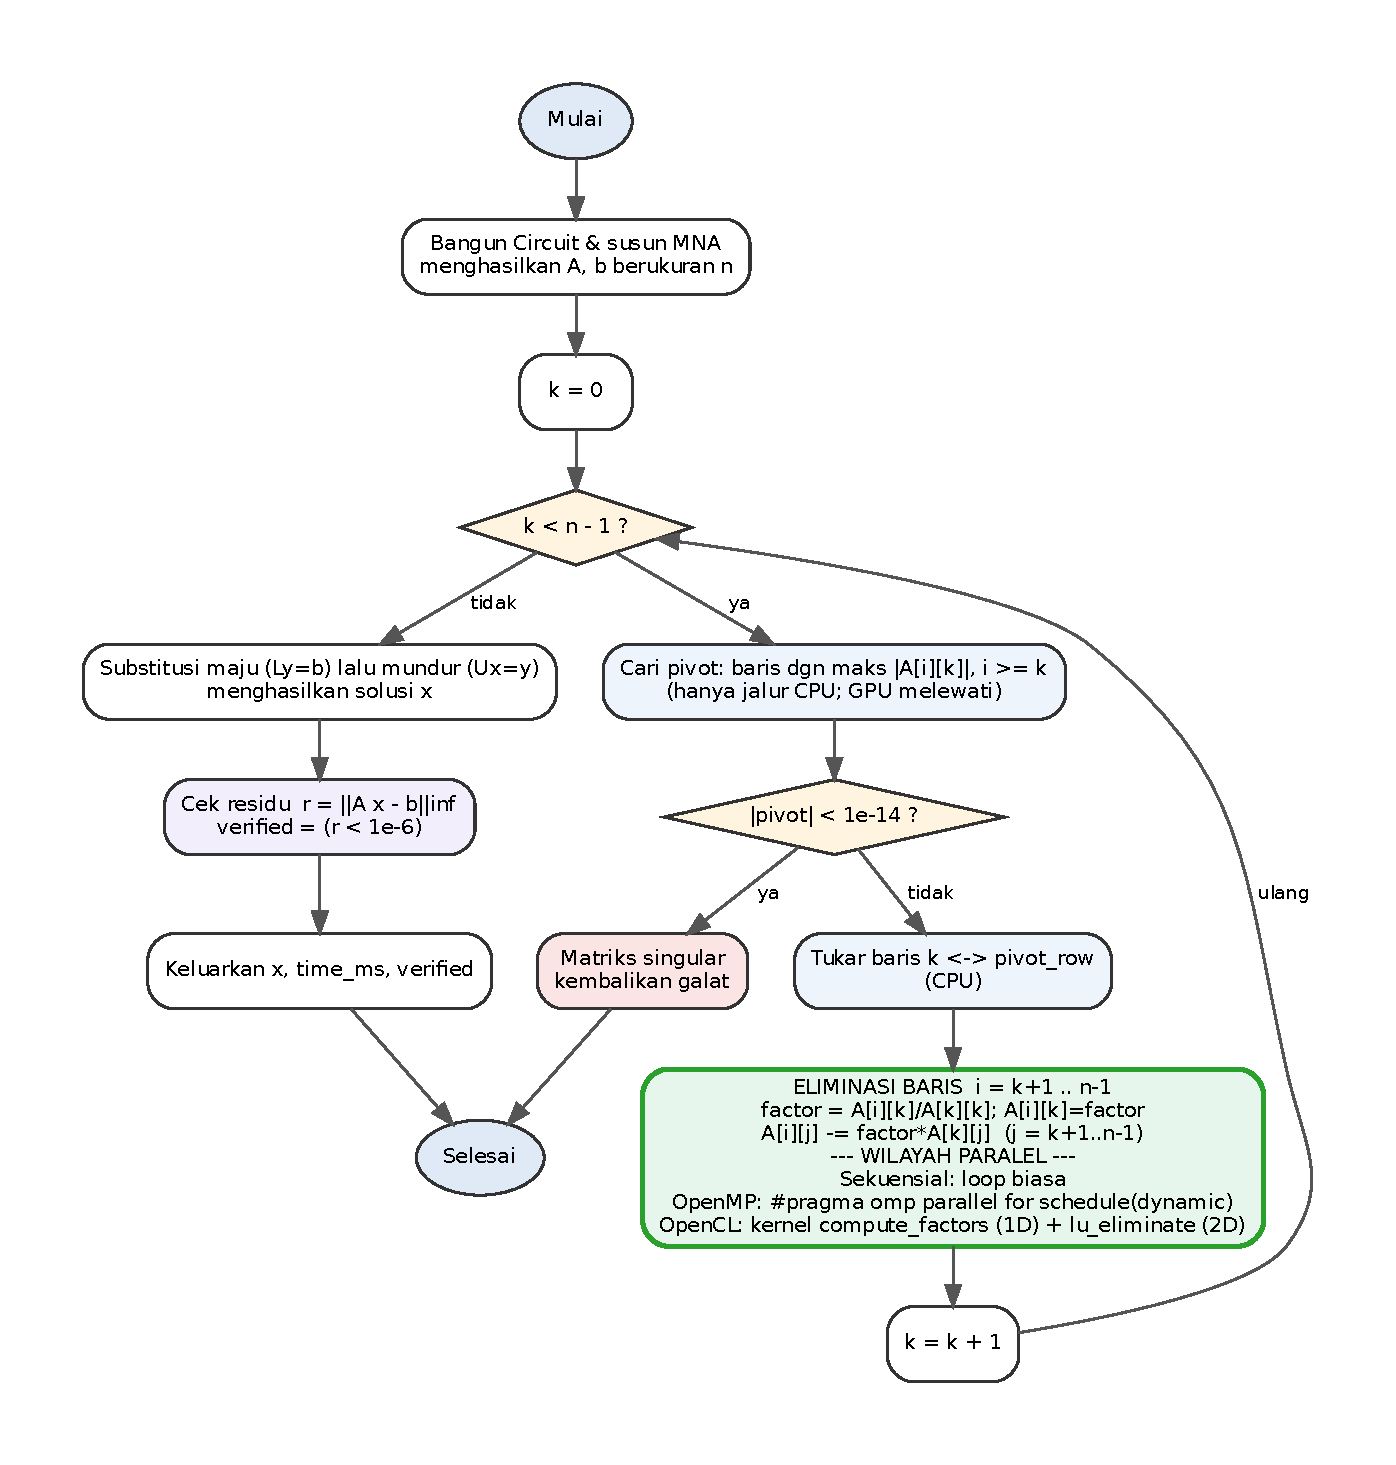
\includegraphics[height=0.92\textheight,width=\columnwidth,keepaspectratio]{fig/flow.pdf}
\caption{Diagram alir solver LU. Blok eliminasi baris (kotak hijau) merupakan wilayah paralel yang diimplementasikan berbeda pada tiap backend.}
\label{fig:flow}
\end{figure}

%==============================================================
\section{Implementasi}
%==============================================================
\subsection{Lingkungan dan Perkakas}
Solver ditulis dalam C++17 dan dikompilasi dengan \texttt{g++} ($-O2$). Paralelisme CPU memakai OpenMP ($-$\texttt{fopenmp}), sedangkan paralelisme GPU memakai OpenCL~1.2. Sistem \emph{build} berbasis \texttt{Makefile} yang mendeteksi keberadaan SDK OpenCL secara otomatis; bila SDK tidak tersedia, sebuah \emph{stub} ditautkan sehingga program tetap dapat dikompilasi dan solver GPU melaporkan diri sebagai tidak tersedia saat dijalankan. Antarmuka baris perintah menyediakan mode \texttt{--test} (validasi), \texttt{--bench N} (uji kinerja), dan \texttt{--compare} (pembandingan terhadap berkas referensi).

\subsection{Backend OpenMP}
Implementasi OpenMP menambahkan satu direktif pada perulangan eliminasi baris, sebagaimana Listing~\ref{lst:omp}. Karena iterasi atas indeks baris $i$ saling bebas dalam satu langkah kolom, perulangan ini aman diparalelkan. Pencarian pivot dan penukaran baris tetap dijalankan sekuensial; bagian sekuensial inilah yang membatasi percepatan sesuai hukum Amdahl~\cite{amdahl1967}. Klausa \texttt{schedule(dynamic)} dipilih agar beban tetap seimbang ketika sub-matriks menyusut pada iterasi $k$ yang besar.

\begin{lstlisting}[language=C++,caption={Wilayah paralel OpenMP (\texttt{lu\_openmp.cpp}).},label={lst:omp}]
#pragma omp parallel for schedule(dynamic) num_threads(nt)
for (int i = k+1; i < n; ++i) {
  double factor = A[i][k] / A[k][k];
  A[i][k] = factor;            // simpan pengali (L)
  for (int j = k+1; j < n; ++j)
    A[i][j] -= factor * A[k][j];
  b[i] -= factor * b[k];
}
\end{lstlisting}

\subsection{Backend OpenCL}
Backend GPU melakukan inisialisasi sekali (memilih perangkat GPU, atau CPU sebagai cadangan, lalu mengompilasi kernel), kemudian menyelesaikan sistem dengan menyalin matriks ke memori GPU dan menjalankan dua kernel untuk tiap kolom pivot $k$:
\begin{itemize}
\item \texttt{compute\_factors} (kernel 1D, $n-k-1$ \emph{work-item}) menghitung pengali $f_i=A_{ik}/A_{kk}$ dan menyimpannya kembali ke bagian segitiga bawah $A$ sebagai faktor $L$;
\item \texttt{lu\_eliminate} (kernel 2D, $(n-k-1)^2$ \emph{work-item}) memperbarui setiap sel sub-matriks aktif, satu sel per \emph{work-item}.
\end{itemize}
Kernel eliminasi inti ditunjukkan pada Listing~\ref{lst:cl}. Substitusi maju-mundur dilakukan kembali di CPU. Karena jalur GPU tidak melakukan pivoting, setiap hasil diverifikasi melalui residu $\lVert A\mathbf{x}-\mathbf{b}\rVert_\infty$; ambang $10^{-6}$ menandai solusi yang sah.

\begin{lstlisting}[language=C,caption={Kernel eliminasi GPU (\texttt{lu\_eliminate.cl}).},label={lst:cl}]
int i = get_global_id(0);  // offset baris dari k+1
int j = get_global_id(1);  // offset kolom dari k+1
int row = i + k + 1, col = j + k + 1;
if (row >= n || col >= n) return;
A[row*n + col] -= factors[i] * A[k*n + col];
\end{lstlisting}

\subsection{Pengukuran Waktu}
Waktu eksekusi CPU diukur dengan \texttt{std::chrono::high\_resolution\_clock}, sedangkan waktu komputasi GPU diukur melalui \emph{event profiling} OpenCL beresolusi nanodetik. Untuk GPU dibedakan \emph{waktu komputasi} (hanya kernel) dan \emph{waktu total} (komputasi ditambah transfer data). Tiap konfigurasi dijalankan lima kali dan waktu \emph{minimum} dilaporkan guna meredam fluktuasi akibat penjadwalan sistem operasi.

%==============================================================
\section{Hasil dan Analisis}
%==============================================================
\subsection{Validasi Kebenaran}
Suite validasi menguji tiga rangkaian dengan jawaban analitik yang diketahui: pembagi tegangan ($1{,}667$ V, $3{,}333$ V, $5$ V), loop sederhana ($I=2$ A), dan tangga 10-tahap. Seluruhnya LULUS. Selain itu, netlist tangga dan \emph{mesh} $3\times3$ diekspor dan disimulasikan pada LTspice; berkas log menunjukkan iterasi titik kerja (\emph{.op}) berhasil pada kedua topologi (ukuran matriks 7 dan 9). Kesesuaian ini memberi keyakinan bahwa pembangun MNA benar tidak hanya pada rantai sederhana tetapi juga pada topologi dua dimensi.

\subsection{Hasil \emph{Benchmark}}
Tabel~\ref{tab:hasil} merangkum waktu eksekusi dan percepatan untuk $n$ dari $51$ hingga $1001$, dan Gambar~\ref{fig:speedup} memvisualisasikan kurva percepatannya. Percepatan didefinisikan sebagai $S = t_\mathrm{seq}/t$.

\begin{table*}[t]
\caption{Waktu Eksekusi (ms) dan Percepatan terhadap Sekuensial}
\label{tab:hasil}
\centering
\renewcommand{\arraystretch}{1.2}
\begin{tabular}{@{}r r r r r r r r r@{}}
\toprule
$n$ & $t_\mathrm{seq}$ & $t_\mathrm{omp4}$ & $S_\mathrm{omp2}$ & $S_\mathrm{omp4}$ & $S_\mathrm{omp,maks}$ & $t_\mathrm{ocl}$ & $S_\mathrm{ocl,komp}$ & $S_\mathrm{ocl,total}$ \\
\midrule
51   & 0{,}027  & 1{,}569  & 0{,}02 & 0{,}02 & 0{,}01 & 2{,}316  & 0{,}01 & 0{,}01 \\
101  & 0{,}189  & 3{,}113  & 0{,}10 & 0{,}06 & 0{,}02 & 4{,}345  & 0{,}04 & 0{,}04 \\
201  & 1{,}705  & 6{,}923  & 0{,}31 & 0{,}25 & 0{,}10 & 11{,}390 & 0{,}15 & 0{,}15 \\
301  & 5{,}253  & 11{,}693 & 0{,}56 & 0{,}45 & 0{,}19 & 16{,}216 & 0{,}32 & 0{,}32 \\
501  & 26{,}684 & 24{,}166 & 1{,}03 & 1{,}10 & 0{,}55 & 33{,}102 & 0{,}81 & 0{,}78 \\
701  & 72{,}265 & 44{,}505 & 1{,}38 & 1{,}62 & 0{,}97 & 56{,}838 & 1{,}27 & 1{,}22 \\
1001 & 247{,}996& 93{,}928 & 1{,}87 & \textbf{2{,}64} & 1{,}85 & 105{,}434 & \textbf{2{,}35} & 2{,}25 \\
\bottomrule
\end{tabular}
\end{table*}

\begin{figure}[t]
\centering
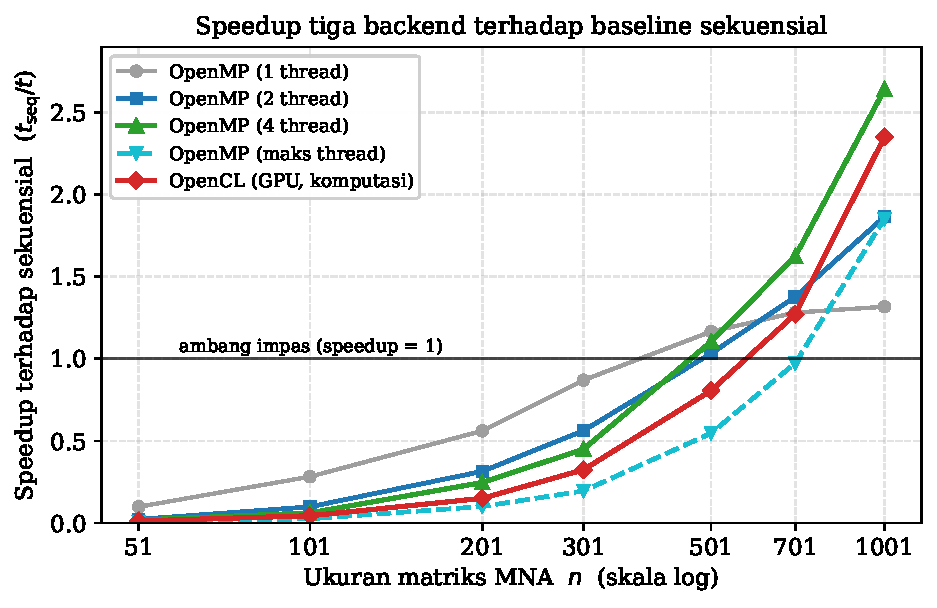
\includegraphics[width=\columnwidth]{fig/speedup.pdf}
\caption{Kurva percepatan tiga backend. Garis impas (\emph{speedup}~$=1$) memisahkan wilayah rugi (atas-kiri) dari wilayah untung (kanan).}
\label{fig:speedup}
\end{figure}

\subsection{Analisis}
\textbf{Fenomena \emph{crossover}.} Untuk matriks kecil ($n \le 301$) seluruh backend paralel jauh lebih lambat daripada sekuensial---hingga puluhan kali lipat. Penyebabnya adalah \emph{overhead} paralelisasi: biaya pembuatan dan sinkronisasi utas pada OpenMP, serta biaya transfer data dan peluncuran kernel pada OpenCL, melampaui beban komputasi sesungguhnya yang masih ringan. Ketika $n$ membesar, beban $O(n^3)$ tumbuh jauh lebih cepat daripada \emph{overhead} yang relatif tetap, sehingga paralelisasi mulai menguntungkan di sekitar $n=500$--$700$ dan mencapai puncaknya pada $n=1001$. Inilah pelajaran inti komputasi performa tinggi: \emph{paralelisasi tidak datang tanpa ongkos, dan baru unggul ketika persoalan cukup besar}.

\textbf{Empat utas mengungguli utas maksimum.} Terdapat hasil yang menarik: pada $n=1001$, OpenMP dengan 4 utas ($2{,}64\times$) justru lebih cepat daripada OpenMP dengan utas maksimum ($1{,}85\times$). Hal ini mengindikasikan bahwa menambah utas melewati titik tertentu malah merugikan, karena tahap eliminasi bersifat \emph{memory-bound}---setiap utas membaca baris matriks secara beruntun dari memori---sehingga utas-utas tambahan justru saling berebut \emph{bandwidth} memori dan menimbulkan \emph{overhead} penjadwalan serta kemungkinan \emph{oversubscription} pada inti logis (\emph{hyperthread}). Temuan ini menegaskan bahwa skalabilitas paralel dibatasi oleh sumber daya bersama, bukan semata jumlah utas.

\textbf{Ongkos transfer GPU.} Percepatan OpenCL berdasarkan waktu total ($2{,}25\times$) sedikit lebih rendah daripada berdasarkan waktu komputasi ($2{,}35\times$) akibat transfer data host$\leftrightarrow$device. Selisihnya kecil karena faktorisasi $O(n^3)$ jauh mendominasi transfer $O(n^2)$, tetapi tetap memperlihatkan bahwa transfer data merupakan komponen biaya nyata pada komputasi GPU.

\textbf{Kompromi tanpa pivoting pada GPU.} Jalur GPU sengaja melewati pivoting parsial karena operasi penukaran baris sukar diparalelkan efisien di GPU. Untuk rangkaian tangga yang \emph{well-conditioned}, pivoting tidak pernah benar-benar diperlukan sehingga solusi GPU tetap benar---dibuktikan oleh cek residu yang selalu lolos. Cek residu inilah jaring pengaman yang akan menangkap kasus apabila pelewatan pivoting menimbulkan ketakstabilan.

\textbf{Keterbatasan.} Sebagai catatan metodologis, matriks MNA dari rangkaian tangga sesungguhnya bersifat jarang (tridiagonal berbatas). Solver jarang atau algoritma Thomas dapat menyelesaikannya dalam orde mikrodetik, jauh lebih cepat daripada ketiga solver padat ini. Dengan kata lain, rangkaian tangga di sini berperan sebagai pembangkit matriks padat berukuran sembarang untuk menguji ketiga backend; angka percepatan yang dilaporkan menggambarkan kinerja \emph{dekomposisi LU padat}---kernel LINPACK kanonik---dan bukan cara tercepat mensimulasikan rangkaian spesifik tersebut. Pemilihan algoritma yang tepat dapat mengungguli paralelisasi algoritma yang keliru.

%==============================================================
\section{Kesimpulan}
%==============================================================
Makalah ini memaparkan rancangan, implementasi, dan analisis sebuah solver rangkaian MNA yang menyelesaikan sistem linear $A\mathbf{x}=\mathbf{b}$ dengan tiga strategi: sekuensial, paralel OpenMP, dan paralel OpenCL. Kebenaran solver tervalidasi terhadap nilai analitik dan terhadap LTspice. Pengujian kinerja memperlihatkan fenomena \emph{crossover} yang khas: paralelisasi merugikan untuk matriks kecil namun menguntungkan untuk matriks besar, dengan percepatan tertinggi $2{,}64\times$ (OpenMP 4 utas) dan $2{,}35\times$ (OpenCL) pada $n=1001$. Analisis lebih lanjut mengungkap dua pelajaran penting: skalabilitas paralel dibatasi oleh \emph{bandwidth} memori (sehingga utas berlebih dapat merugikan), dan akselerasi perangkat keras tidak menggantikan pemilihan algoritma yang tepat. Sebagai pengembangan, solver dapat diperluas dengan jalur algoritma Thomas/jarang sebagai pembanding, peluncuran kernel berkelompok untuk menekan \emph{overhead} GPU, serta uji kasus matriks ber-\emph{pivot} guna menguji ketahanan jalur GPU yang tanpa pivoting.

%==============================================================
\begin{thebibliography}{9}
\bibitem{nagel1975spice}
L. W. Nagel, ``SPICE2: A computer program to simulate semiconductor circuits,'' Univ. California, Berkeley, Tech. Rep. ERL-M520, 1975.

\bibitem{ho1975mna}
C.-W. Ho, A. E. Ruehli, and P. A. Brennan, ``The modified nodal approach to network analysis,'' \emph{IEEE Trans. Circuits Syst.}, vol. 22, no. 6, pp. 504--509, Jun. 1975.

\bibitem{golub2013matrix}
G. H. Golub and C. F. Van Loan, \emph{Matrix Computations}, 4th ed. Baltimore, MD, USA: Johns Hopkins Univ. Press, 2013.

\bibitem{dongarra2003linpack}
J. J. Dongarra, P. Luszczek, and A. Petitet, ``The LINPACK benchmark: Past, present and future,'' \emph{Concurrency Comput., Pract. Exper.}, vol. 15, no. 9, pp. 803--820, 2003.

\bibitem{davis2010klu}
T. A. Davis and E. Palamadai Natarajan, ``Algorithm 907: KLU, a direct sparse solver for circuit simulation problems,'' \emph{ACM Trans. Math. Softw.}, vol. 37, no. 3, pp. 1--17, 2010.

\bibitem{dagum1998openmp}
L. Dagum and R. Menon, ``OpenMP: An industry standard API for shared-memory programming,'' \emph{IEEE Comput. Sci. Eng.}, vol. 5, no. 1, pp. 46--55, Jan.--Mar. 1998.

\bibitem{stone2010opencl}
J. E. Stone, D. Gohara, and G. Shi, ``OpenCL: A parallel programming standard for heterogeneous computing systems,'' \emph{Comput. Sci. Eng.}, vol. 12, no. 3, pp. 66--73, May--Jun. 2010.

\bibitem{amdahl1967}
G. M. Amdahl, ``Validity of the single processor approach to achieving large scale computing capabilities,'' in \emph{Proc. AFIPS Spring Joint Comput. Conf.}, 1967, pp. 483--485.
\end{thebibliography}

\end{document}